\chapter{Methodology}

\section{Canonical Action Research (CAR)}

% Give more comparison between original Action Research vs Canonical Action Research

\paragraph{} For this study, Canonical Action Research (CAR) was the research methodology used to examine the implications of practicing a cooperative game development model and to facilitate improvement and iteration. CAR is a cyclical model of study on the application and practical consequences of enabled action through iteration and collaboration to facilitate change. The researcher works directly with the participants to plan and execute an action, collect their feedback on it and iterate upon that action; this action is centered around a researched and applied theory. The CAR process model consists of exploring the problem, diagnosing that problem, planning the action, executing that action, evaluating its successes and failures, and improving that action through reflection and analysis \autocite{davison_principles_2004}.

\paragraph{} CAR is an extension of the Action Research methodology first described by Kurt Lewin in 1944. Lewin's Action Research studies the effects of various forms of social action through collaboration with participants to understand how organizational change can be facilitated. This methodology uses a repetitive process of strategizing, implementing an action, and fact-finding through the analysis of that action to achieve those ends. The goal of Action Research is to encourage some form of change; the methodology uses the action to study the effects of the change and what could be done to further improve its facilitation. This methodology is primarily considered with the study of the relation between possible conditions and results in relation to the diagnosis of a particular situation \autocite{lewin_action_1946}.

\paragraph{} CAR builds upon Lewin's methodology by emphasizing rigor through iteration as a form of intervention, and continuous problem diagnosis through participation. By cyclically improving the action, the researcher is repeatedly engaged in the analysis necessary for knowledge-building to take place. CAR differentiates itself from Lewin's Action Research in that the interventions must be more adaptable because the repetition of engagement constantly reshapes the circumstances. This lack of complete control requires the researcher be flexible in their approach to action which may not be necessary for other types of Action Research methodologies.\autocite{davison_principles_2004}.

\paragraph{} CAR is applicable to the study of cooperative game development because of its emphasis on change through action. This study seeks to examine how cooperativism can be applied to game development by creating a viable production model for cooperative teams that can facilitate consensus-building and creative collaboration. Game development as heterogeneous engineering produces an artifact as an output and as such the processes by which that artifact is created can be studied. CAR is appropriate for the study because it allows the researcher to directly observe and engage with the participants developing games using the actionable model. The researcher can intervene and iterate to improve the model such that it may encourage teams of game developers to pursue cooperative forms of production.

\paragraph{} CAR consists of seven processes, five of which are part of the iterative cycle. The start and end of the study are defined by an entrance and exit. During the entrance, the researcher identifies the problems studies the theory being applied and previous attempts to solve the problem. In CAR, applying the theory to the action is essential for knowledge-building as it offers potential solutions. At the end of the iterative cycle, the researcher exits by analyzing their work and considering further implications. These are the only two CAR processes not subject to iteration as they mark the beginning and end of the study \autocite{davison_principles_2004}.

\begin{figure}[h!]
    \centering
    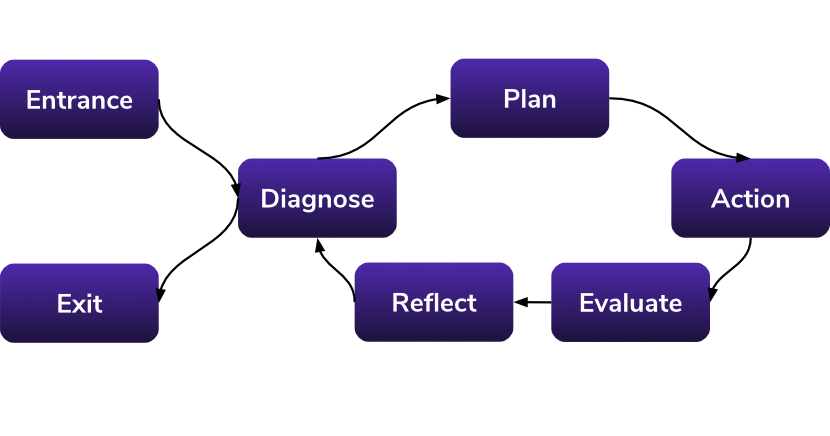
\includegraphics[width=\linewidth]{Figures/CAR.png}
    \caption{The seven processes of the cyclical model of CAR.}
\end{figure}

\paragraph{} The first two processes of the iterative cycle of CAR are diagnosis and planning. During the diagnosis phase, the researcher examines the nature of the problems being addressed and the situational needs of the study based on the previous iteration if applicable. This take place independently of any diagnostics by the participants such that the researcher can determine an appropriate intervention. The assessments that result from that inform the planning of how the action will take place. This plan should reflect the refinements made to understand the applied theory \autocite{davison_principles_2004}.

\paragraph{} The essence of all forms of Action Research is the execution of the planned action with the study participants \autocite{lewin_action_1946}. The rigor of CAR is derived from the direct engagement of the researcher with the participants through the repeated implementation and iteration on the action. The researcher through participation can observe and experience the action as it is taking place; this acts as a form of data collection for the analysis of the actions or its implications. This might require an agent who can help facilitate the intervention but is not always necessary. \autocite{davison_principles_2004}.

\paragraph{} The final two processes of CAR are the collection and analysis of data surrounding the executed action. In addition to the observational and experiential data derived from the researcher participating in the action, they may also collect qualitative or quantitative data to inform decisions surrounding the next iteration. In addition, the theory should also inform the analysis as the study of the action is centered around it. By reflecting and analyzing the data, the researcher decides which aspects of the action worked and which are to be discarded. After this, the CAR cycle repeats until the research exits the study \autocite{davison_principles_2004}.

\paragraph{} CAR also consists of five principles, the first which is the Principle of Researcher-Client Agreement; this criteria establishes internal validity among shareholders through reciprocal assurances of behavior, and agreed-upon data-collection methodologies. The second principle, the Principle of the Cyclical Process Model, is embodied through the repeated iterations of diagnosis, planning, action, assessment and reflection. The application of the theory to the enabled action is the Principle of the Theory as described by CAR and defines the goals of the project and subsequently the shape of the action. The Principle of Change through Action reflects the essence of CAR as it seeks to change the current situation, a lack of which makes the action taking place meaningless. Finally, the analysis of the data, consideration of implications, and the improvement of the action from that analysis comprise the Principle of Learning through Reflection that enables the knowledge-building aspects of CAR \autocite{davison_principles_2004} 

\paragraph{} When synthesized together, these processes and principles are applied to analyze implementing a game development model for cooperative teams to form this study. The study started by examining problems in cooperative game development and researching the underlying theory behind cooperative organizations. The cyclical model of iteration was applied to using a cooperative game development model and feedback was collected from participants to improve it. The feedback analysis was subsequently reflected in the incremental changes to the model and its implications later discussed.

\paragraph{} The study consisted of the researcher working with a group of four undergraduate students over approximately six weeks to create a game using a cooperative production model that would be improved by the researcher after collecting feedback from the participating students. The group consists of students creating a game for a final project of an undergraduate game design course with each having their own unique skill set. In addition to developing and facilitating the model, the researcher also provided technical assistance in tutoring and guidance to help the team of students fix issues that might arise during development. As a member of the team as permitted by CAR, the researcher also contributed to the decisions alongside the participating student developers.

\paragraph{} Feedback was collected from the cooperative team through interviews, observations and anonymous surveys. One-on-one interviews were conducted with each member to get their prospective on the model, working in a cooperative team and their thoughts for improving the action. Anonymous surveys were used to offer additional insights that might not be exposed during the interviews due to the researcher being personally engaged with the participants. The researcher also observed the application of the model as a direct participant in the study.

\section{Design Component}

\paragraph{} The design component of this study is a game development model for cooperative teams of developers. The term "model" refers to the description of steps and strategies that apply cooperativism to facilitate game development on democratic teams. This model uses principles of cooperativism as a framework for fostering collective decision-making in the game development process. When applied, these principles also serve as a means of mitigating or solving social issues that often present themselves among teams of developers making games. The goal of designing this model is to study how cooperativism can be applied to game development to create a viable production model for cooperative teams developing games. In accordance with the research framework used for the study, CAR, the model was developed iteratively over the course of six weeks with a group of undergraduate university students, alongside the researcher, working on a game for the final project of a course.

\paragraph{}

\begin{figure}[h!]
    \centering
    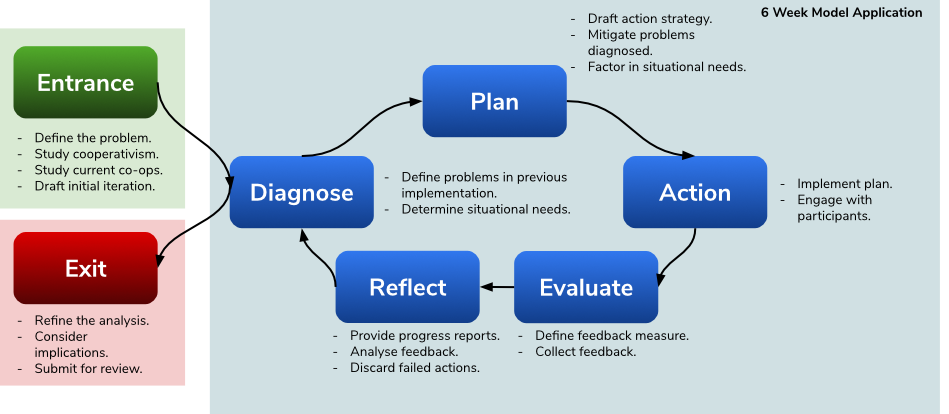
\includegraphics[width=\linewidth]{Figures/AppliedCAR.png}
    \caption{The seven processes of CAR as applied to this study.}
\end{figure}

\paragraph{} The model uses the tenets of cooperativism to address the social problems that arise in game development. Cooperativism is able to address issues of alignment on teams by facilitating cross-education between members. Additionally, the consensus necessary for decisions to be made in a cooperative teams act as another form of alignment. Participation and personal investment among the team are encouraged through cooperativism because developers are owners and managers of the game. The model implements these tenets through actionable steps cooperative teams can take when developing a game. 

\paragraph{} The first iteration of the model emphasized the facilitation of democratic decision-making through explicit synchronization on goals and tasks. It focused on alignment of members through laying out the game's goals, members' needs, desired featured, and tasks before executing on production. Concensus was central to this iteration of the model as it served as the basis for aligning each developer. Although not explicitly accentuated, communication among members was a vital attribute to solidifying synchronicity with frequent contact encouraged.

\begin{figure}[h!]
    \centering
    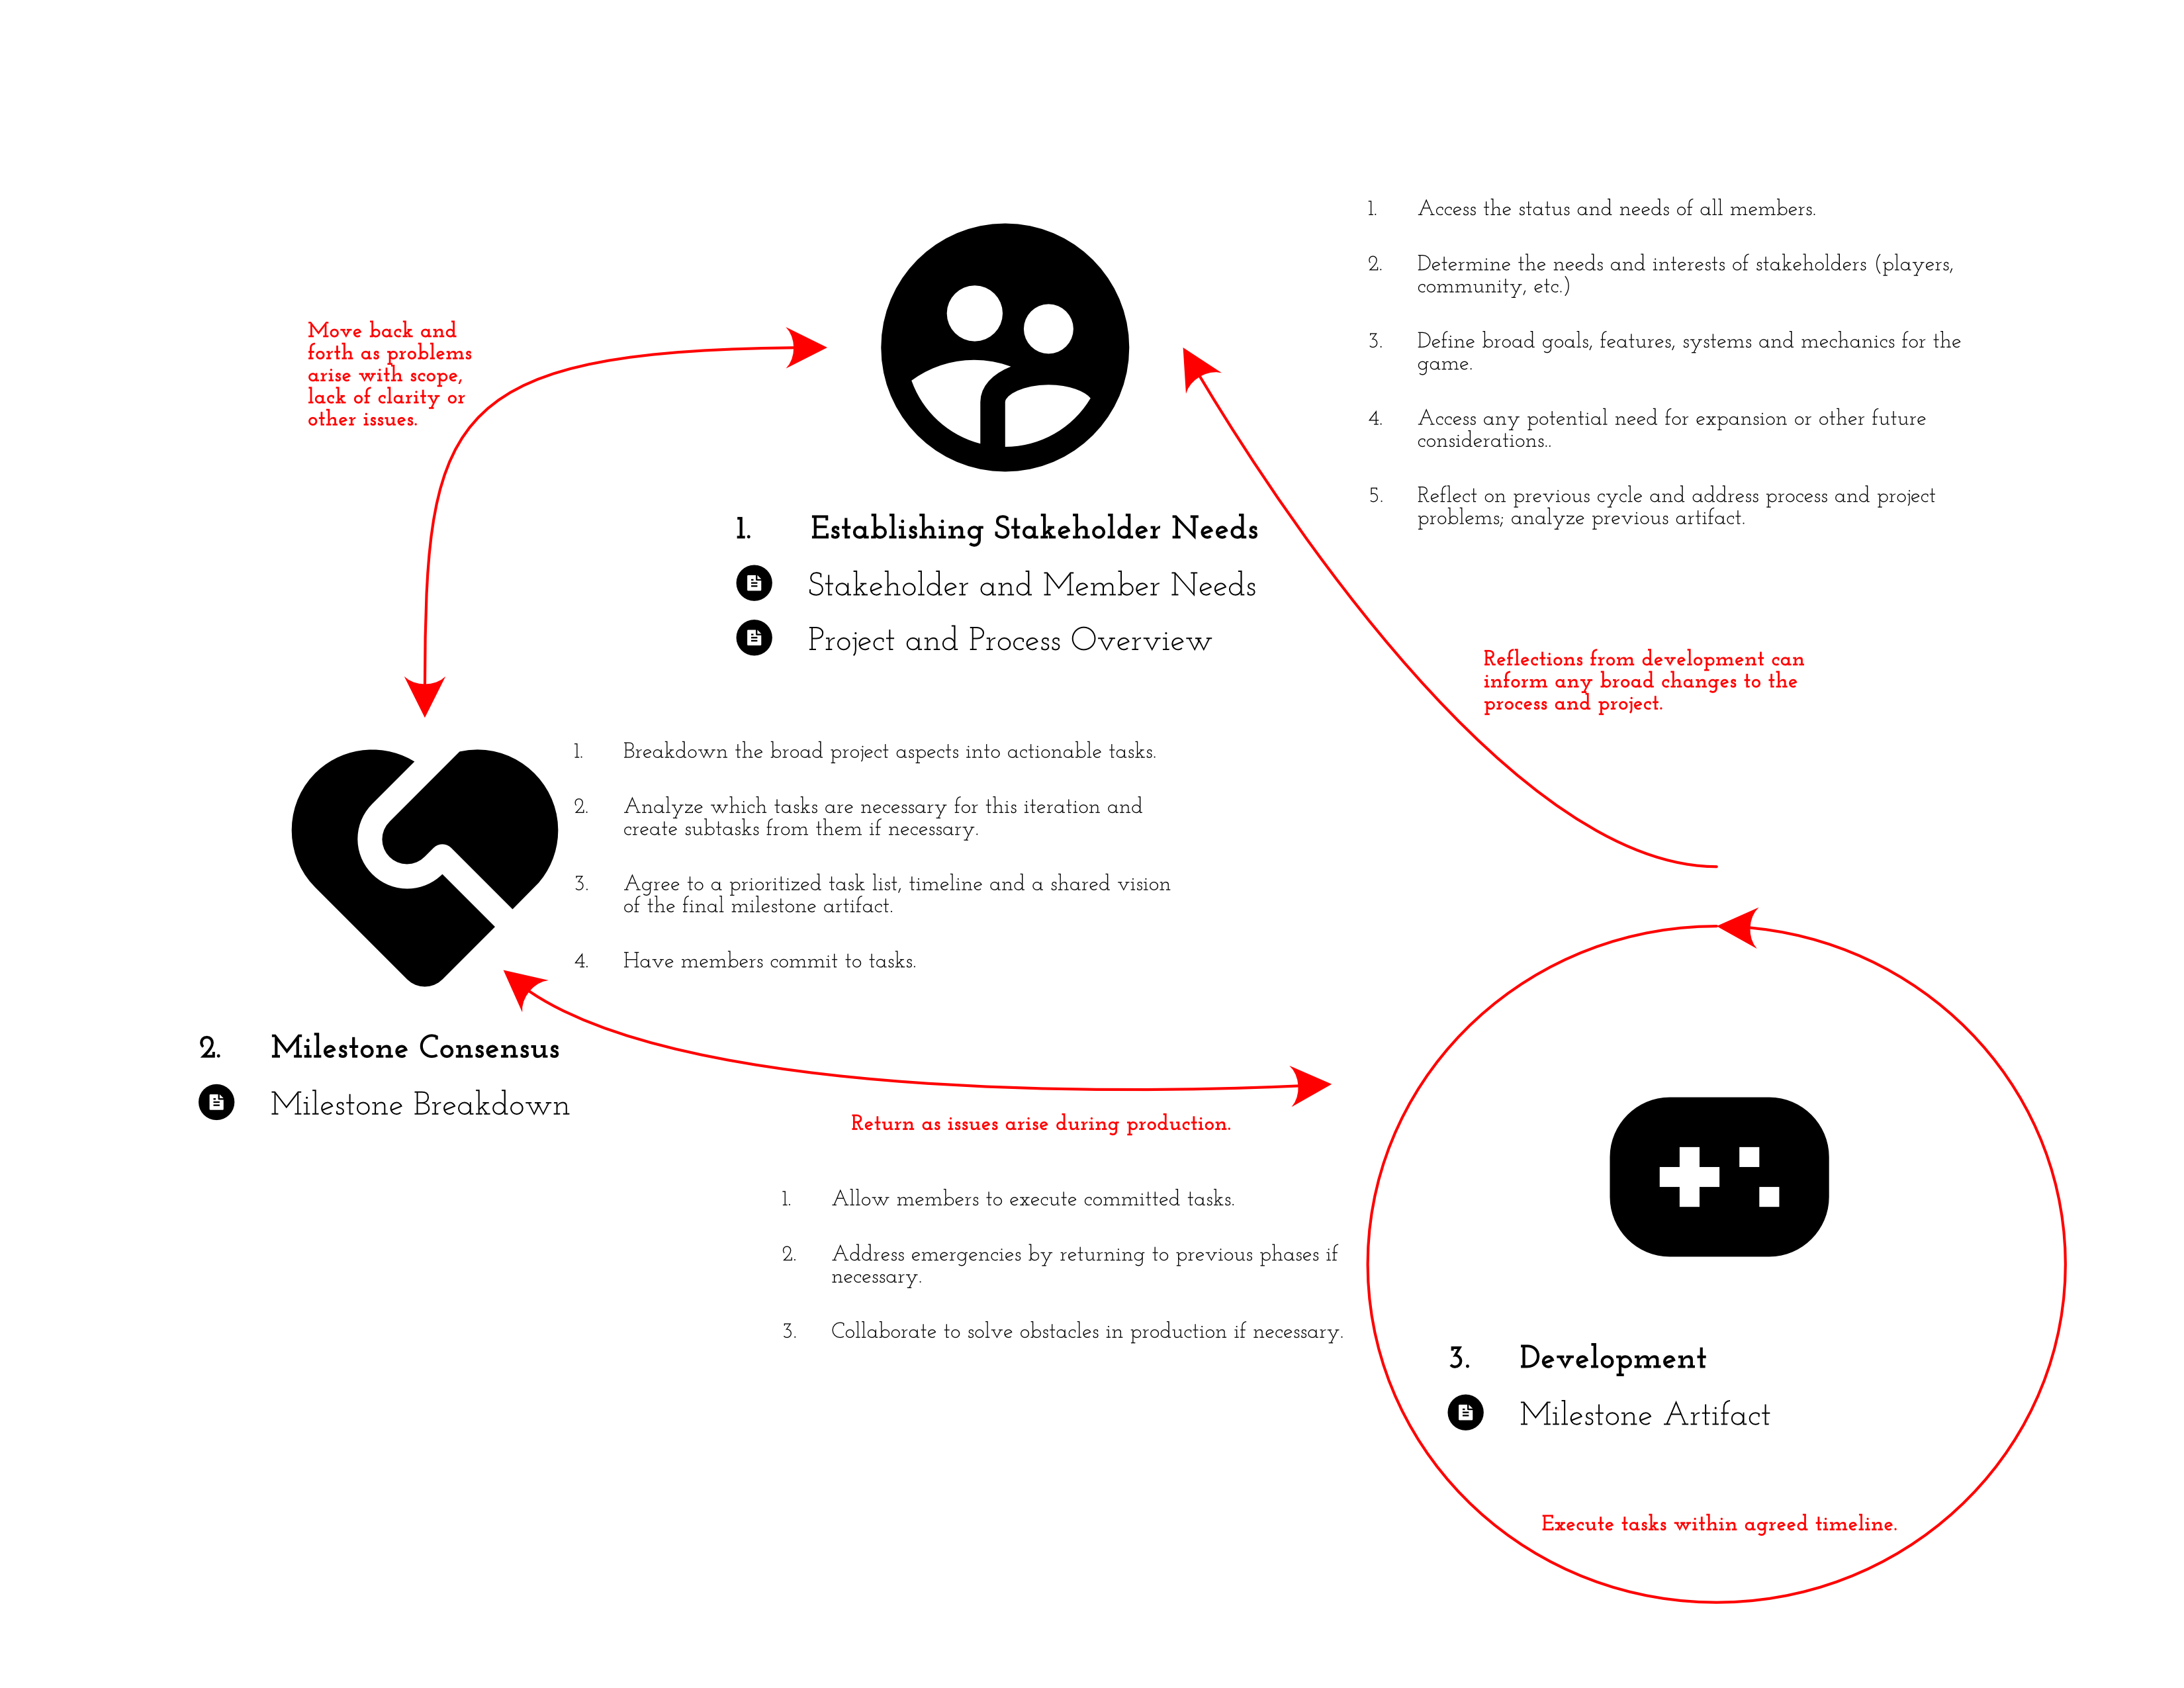
\includegraphics[width=\linewidth]{Figures/FirstModel.png}
    \caption{The first iteration of the model.}
\end{figure}


\paragraph{} This iteration of the model was significantly changed as a result of the research for this study. It was created to explicitly denote when alignment needed to occur within the game development process; however, data from the participants and additional research into cooperative game development exposed the flaws in this approach. One of such flaws was that the model was based on developers needing to know when a vote or alignment was necessary. In the case of the cooperative group apart of the study, this was more intuitive for them than the model accounted for. Additional research on cooperative game studios also contributed to this insight with members of co-ops noting that more issues persisted with communication than when to vote.

\paragraph{} Another flaw of the first model was that it failed to leverage a vital tenet of cooperativism: education and information-sharing among members. While the facilitation of democratic decision-making was present, the model did not take into account how interpersonal relations between developers and their tools impacts the process by which decisions are made. The model made clear when collective decision-making needed to occur but it did not consider the circumstances that shape how those decisions occur. This insight was exposed by comparing the research done on the social problems of game development, the principles of cooperativism, the experiences of game co-op developers and the model as it was currently constituted; communication and cross-education were vital to both cooperative management and game development but the model did not address either.

\paragraph{} Thus from this a second model was created, the core of which persisted throughout the remainder of the study. Rather than defining clear points in the game development process where decisions needed to be made, this iteration of the model deviated towards building the type of game development environment necessary for cooperative teams to be aligned and participatory. The goal of the model transitioned away from simply being about cooperation through the ability to vote to being about cooperation through being empowered with the conditions necessary to make meaningful decisions with the team. This led to the restructuring the model around three key components necessary for cooperative decision-making: communication, synchronization, and collaboration.

\begin{figure}[h!]
    \centering
    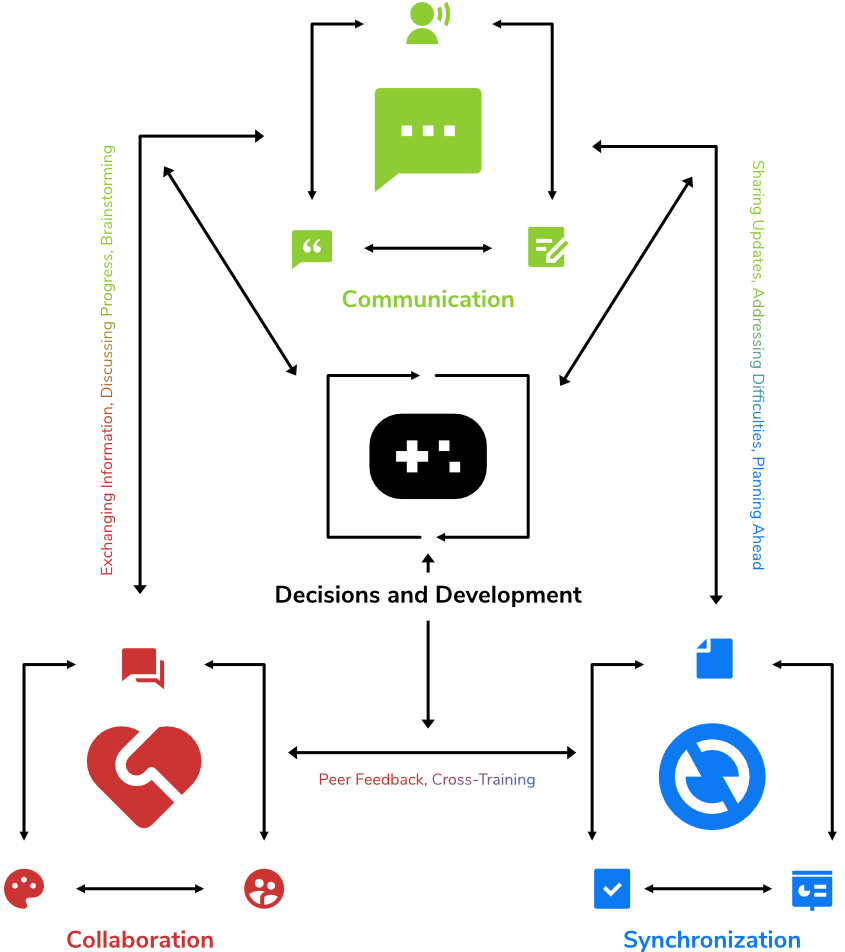
\includegraphics[width=\linewidth]{Figures/Model.png}
    \caption{The final iteration of the model; the structure was introduced in the second iteration.}
\end{figure}

\paragraph{} One of the three core components of the model is communication. The facilitation of joint ownership requires those owners be able to share information with one another effectively and efficiently. Dialogue is essential for aligning the goals of the team and forming a consensus around decisions effecting the production; this was emphasized by the game co-op members who spoke at GDC 2019 \autocite{game_developers_conference_embracing_2019}. Each member's degree of participation in conversation may depend on their sociality. This also includes conversations that should need to take place among individual members who may need to collaborate or share information. Communication in cooperative game development teams can be accomplished through meetings, frequent progress updates, and brake-out sessions.

\paragraph{}

\begin{figure}[h!]
    \centering
    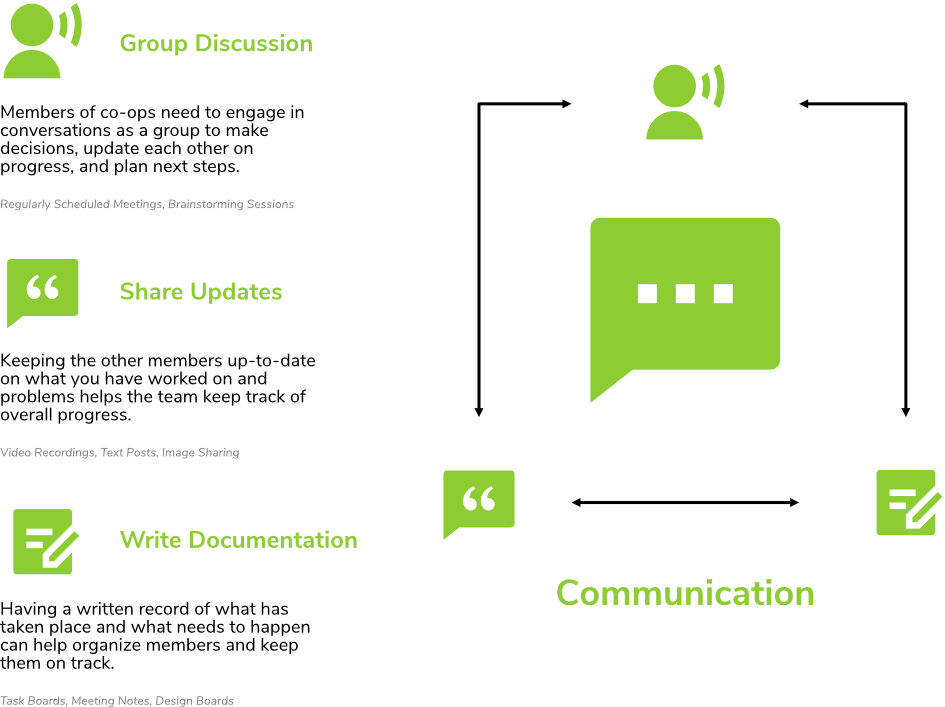
\includegraphics[width=\linewidth]{Figures/Communication.png}
    \caption{The model's strategies for communicating first introduced in the third iteration.}
\end{figure}

\paragraph{} The team for this study used a voice-and-chat app to schedule meetings, update one another on their work, and collaborate in order to communicate with one another. The team had at least two or more groups voice meetings per week in which everyone attend. During those meetings, the team would discuss design decisions in regards to the game's mechanics and art style in addition to alignment on next steps. Voice meetings among smaller subgroups of members also took place where members collaborated or shared knowledge. Screenshots, videos and text-based updates were shared in chat channels so each member could keep each other up-to-date on the progress of their work.

\paragraph{} Communication is vital to cooperative game development teams because it facilitates the exchanging of information necessary for members to make decisions and contribute to production. Open dialogue between members of cooperative teams fosters synchronicity by allowing members to ask questions and give their thoughts as equals. Additionally, it also allows members to express concerns, make proposals or share resources. Frequent communication also helps the developers to form a shared mental model of the tasks and vision of each step of the production process through opportunities to address alignment. These are essential to cooperative game development teams because they define how decisions can be made; it brings each member into the process by giving them the information and voice to empower them to be effective members.

\paragraph{} In addition to communication, synchronization is also a core component of the model. Synchronization consists of aligning each member on the status of the project and sharing information with one another; this is an extension of communication as it focuses on the outcome of knowledge-sharing and establishing shared goals rather than the acts of dialogue that go into it. This component was designed to reflect the educational principle of cooperativism by turning knowledge-sharing into an active goal as part of the game development process. Recommended steps to synchronize members includes creating task boards, cross-training on tools and techniques, and frequently engaging in communication.

\begin{figure}[h!]
    \centering
    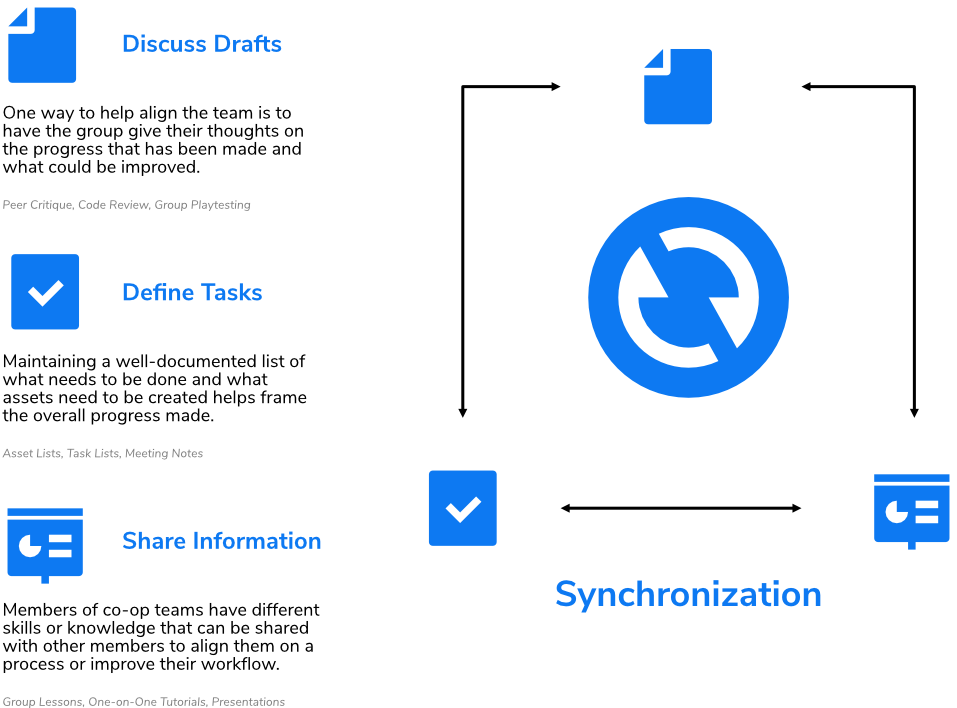
\includegraphics[width=\linewidth]{Figures/Sync.png}
    \caption{The model's strategies for synchronization first introduced in the third iteration.}
\end{figure}

\paragraph{} This was executed as part of the study team through organizational methods such as a voice-and-chat server and a digital task board in addition to interpersonal methods such as one-on-one assistance and resource sharing. The primary means by which the team stayed aligned on tasks and progress was through frequent communication on the voice-and-chat server through meetings and text updates. In terms of education and resource-sharing, the team found that one of the primary places these were most needed was on technical tasks within the game engine. The researcher and two participants primarily responsible for programming and other technical tasks met at least once a week to align on the use of the engine, teach anyone who needed to know how to complete those tasks, and to assist each other with problems that presented themselves as tasks were being completed.

\paragraph{} Synchronization is important for a cooperative game development model to succeed because it informs the possibilities of the collaboration taking place. In the case of the study, the dissection and analysis of the engine and its capabilities helped the members of the team define which features could reasonably be implemented within the timeline and milestones of their course project. This also had the additional benefit of allowing multiple members to be able to reframe those technical limitations in different ways when explaining them to the other members. By achieving alignment, members can make more informed decisions surrounding the game. 

\paragraph{} The third core component of the model is collaboration. One of the unique features of cooperative teams are that they are structurally participatory; decisions are facilitated by collective input and engagement. This collectivism can also be channeled into problem-solving or creative activities through joint work. Members with differing mental models can benefit the work one another by offering a different prospective on engaging with the problem or task. Some strategies for facilitating collaboration among developers in a cooperative group include group design and peer work sessions.

\paragraph{} Collaboration on cooperative teams is unique in that the participatory aspects of the management structure can be used as an asset during creative planning in game development. All the members of these teams are engaged in the decision-making process and as such participation in that can be leveraged to design elements of the game itself. Since game development is multidisciplinary in practice, developers of cooperative teams often have different skills and mental models that can help shape the end result through their contribution. Members of similar skills can also leverage their shared knowledge to collectively solve technical problems that could arise during development.

\paragraph{} These types of sessions were implemented in the study as weekly events where the team got together and ideated on mechanics and created designs for the game in addition into breaking off into smaller groups to work together. The group took advantage of the participation required from cooperative teams by including everyone in the designing of levels and mechanics. This provided different perspectives that were applied to create a designs that all the members were invested in because they contributed to it. These perspectives were also applied in small subgroups of the team where individual members met to solve specific problems with tasks such as unifying the art style or implementing a feature.

\begin{figure}[h!]
    \centering
    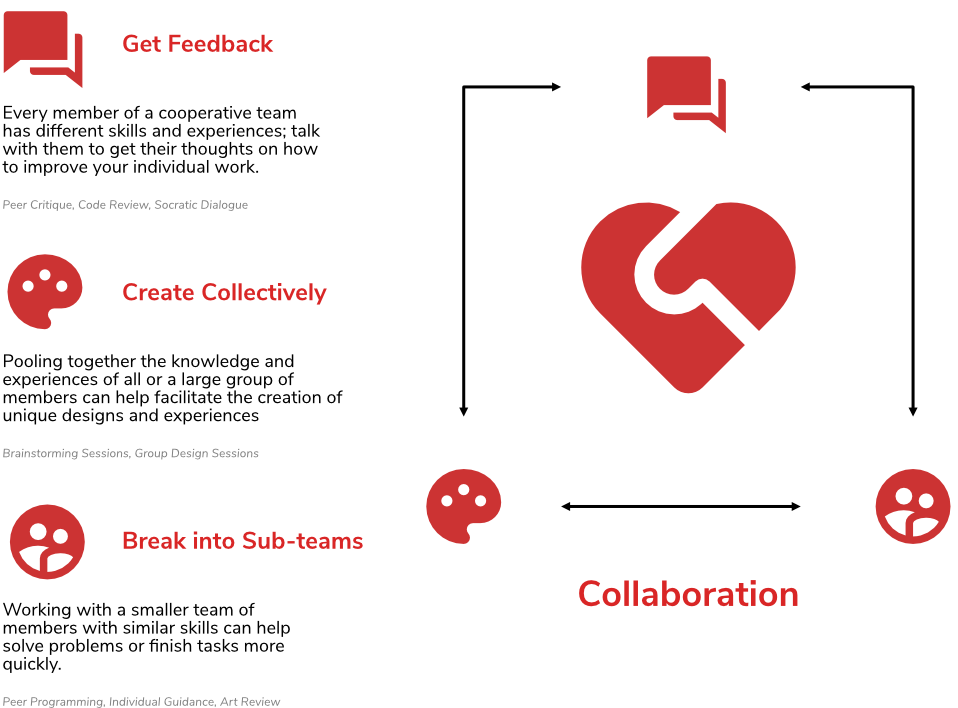
\includegraphics[width=\linewidth]{Figures/Collab.png}
    \caption{The model's strategies for collaboration first introduced in the third iteration.}
\end{figure}

\paragraph{} These three core components synthesize cooperative principles with game development strategies in order to create an environment where democratic teams of developers are empowered to facilitate decision-making and creative collaboration. The communication component is reflective of the principles of member participation and control as exchanging information helps to align members on the status of development. Synchronization is the outcome of educating, training and exchanging of information which are core principles of cooperativism. The member participation and control principles of cooperativism are also applied through the collaboration component where the inclusion of the developers in the decision-making process is used to encourage further participation in creative, technical or other types of problem-solving activities.

\paragraph{} As the second model proved much more successful at applying cooperativism to game development than the first, the third iteration kept the structure of its predecessor and added additional strategies to help members better exercise each component. This was derived from the feedback received; the participants noted that cooperativism empowered them to engage with each component of the model but that a lack of clear strategy sometimes made it difficult to full realize them. The researcher also observed this where members would sometimes lose track of deadlines, miss meetings, or fail to communicate regularly. The third iteration introduced strategies in the form of actionable items that could be implemented as part of each component to help exercise them.